%---------------------------------------------------------------------------------------------------
% Test
%---------------------------------------------------------------------------------------------------
\newpage
\chapter{Test}

After the implementation, the components and the complete unit itself need to be tested. The results are evaluated particularly with regard to the required features.
Table \ref{tab:equipment} shows the laboratory instruments primary used during the testing phase.
Besides a function generator and an audio analyzer as common sources for input signals, the unit is tested with an electric guitar\,(Stratocaster type - single coil pickups with 6 strings). In combination with a guitar amplifier the subjective auditory impression can be evaluated.

\begin{table}[H]
\centering
\begin{tabular}{ll}
	\hline
	\textbf{Instrument} & \textbf{Type}  \\
	\hline
	Peaktech 3500FG & Function Generator  \\
	Tektronik MSO2024 & Oscilloscope  \\
	Rohde \& Schwarz UPV & Audio Analyzer \\
	Harley Benton ST-20 BK & Electric Guitar \\
	Marshall Park G10 & Combo Guitar Amplifier \\
	\hline
\end{tabular}
\caption{Test equipment}
\label{tab:equipment}
\end{table}




\section{Preamp Module Performance}


The preamp module is tested to the two major demands given in the requirements in the first place:
The voltage level adjustment and the voltage bridging. Measured in the time domain with the oscilloscope, the transition of a sine wave is measured. The input signal is provided by the function generator, representing a signal within the voltage- and fundamental frequency-range of an electric guitar. For the inspection of the voltage bridging, the preamp module is tested with and without a connection to the active Audio-HAT (unloaded and loaded).

\subsubsection{Instrument Level to Line Level}

For the amplification path of the preamp module, an input signal with 108\,mV$_{\mathrm{Peak}}$ at 200\,Hz is used.
The measured transition\,(unloaded) from instrument level to line level has a deviation of 3,12\,\% (\ref{tab:Pre-Amplification}), which can be reasoned by production-related deviations of the used parts. For the interconnection with the Audio-HAT, a high voltage transfer is ensured. The signal amplitude is only slightly attenuated by 4,35\,\% as result of suitable voltage bridging(see figure \ref{fig:unloaded} and figure \ref{fig:loaded}).


\begin{table}[H]
\begin{center}
\begin{tabular}{|c|c|c|c|c|}
\hline 
 $U_{\mathrm{INSTRUMENT\_IN}}/\mathrm{mV}$ & $U_{\mathrm{LINE\_OUT}}/\mathrm{mV}$ & $\mathrm{Gain}_{\mathrm{measured}}$ & $\mathrm{Gain}_{\mathrm{implemented}}$ & $\mathrm{deviation}/$\% \\ 
\hline 
108 & 368 & 3,407 & 3,517 & 3,12 \\ 
\hline 
\end{tabular} 
\end{center}
\caption{Measurement of pre-amplification}
\label{tab:Pre-Amplification}
\end{table}

\begin{minipage}[t]{0.5\textwidth}
\includegraphics[width=\textwidth]{Preamp_timedomain/banksy.jpg}
\captionof{figure}{Pre-amplification (unloaded)}
\label{fig:unloaded}
\end{minipage}
\begin{minipage}[t]{0.5\textwidth}
\includegraphics[width=\textwidth]{Preamp_timedomain/banksy.jpg}
\captionof{figure}{Pre-amplification (loaded)}
\label{fig:loaded}
\end{minipage}


\subsubsection{Line Level to Instrument Level}

As an exemplary input signal for the attenuation path 360\,mV$_{\mathrm{Peak}}$ at 200\,Hz is suitable.
For the adjustment of the signal back to instrument level, a minimal deviation of 0.714\,\%\,(\ref{tab:Attenuation}) is achieved.
This is reasonable due to the non-complex used solution as a voltage divider.
An oscilloscope measurement is depicted in figure \ref{fig:Attenuation}.



\begin{table}[H]
\begin{center}
\begin{tabular}{|c|c|c|c|c|}
\hline 
$U_{\mathrm{LINE\_IN}}/\mathrm{mV}$ & $U_{\mathrm{INSTRUMENT\_OUT}}/\mathrm{mV}$ & $\mathrm{Gain}_{\mathrm{measured}}$ & $\mathrm{Gain}_{\mathrm{implemented}}$ & $\mathrm{deviation}/$\%  \\ 
\hline 
360 & 100 & 0,278 & 0,280 & 0,714 \\ 
\hline 
\end{tabular} 
\end{center}
\caption{Measurement of attenuation}
\label{tab:Attenuation}
\end{table}

\begin{figure}[H]
	\centering \includegraphics[width=0.5\textwidth]{Preamp_timedomain/banksy.jpg}
	\caption[Menu]{Attenuation}
	\label{fig:Attenuation}
\end{figure}

\subsubsection{Frequency Response}
% Frequency response and THD
The Audio Analyzer is used for the measurements of the preamp module in the frequency domain. Figure \ref{fig:PreampFreq} shows the frequency response of the amplification path using a sine sweep between 10\,Hz and 20\,kHz. The characteristic flat frequency response of adopted MXR Micro-Amp design is ensured within the range of the fundamental frequencies between 82,41\,Hz and 1318,5\,Hz\,(see section \ref{subsec:FrequencyRange}).
The curve is damped in the range of higher frequencies. The minimal reduction of 4,5\,\% ( $\widehat{=}$ 16\,mV) can be neglected, so the guitar harmonics are appropriately amplified.


\begin{figure}[H]
	\centering \includegraphics[width=0.8\textwidth]{banksy.jpg}
	\caption[Menu]{Preamp frequency response}
	\label{fig:PreampFreq}
\end{figure}

\subsubsection{Total Harmonic Distortion plus Noise}

For the evaluation of the audio performance, the THD+N is measured with the Audio Analyzer.
As a standard for THD+N measurements, a sine-wave signal of 1\,kHz is used. The amplitude is set to 100\,mV$_\mathrm{RMS}$ representing a realistic output of an electric guitar.
The resulting THD+N of -85.003\,dB (0.006\,\%) indicates a very good performance in regard to the desired application field. 

\begin{figure}[H]
	\centering \includegraphics[width=0.5\textwidth]{banksy.jpg}
	\caption[Menu]{Preamp THD+N}
	\label{fig:PreampTHD}
\end{figure}

\subsubsection{Hearable Results}

In a practical test, the isolated preamp module is verified with the usage of the electric guitar signal.
The amplification path is tested in the first place by connecting the \textit{LINE\_OUT} with an AUX(auxiliary) input of HIFI-Amplifier and with the input of a PC-Soundcard. In both cases, the hearable result is a clean undistorted sound from the subjective point of view.
A possible extension for further developments might be a usage of the consumer audio line level outside of the effect unit.\\ 
\\
In a further test, the \textit{LINE\_OUT} is connected directly with \textit{the LINE\_IN} to test the preamp module as a whole.
According to the defined requirements, the total signal processing shall not change the loudness of the guitar signal.
The module is connected via the \textit{INSTRUMENT\_OUT} jack with the Input of the guitar amplifier.
As a hearable result, the guitar-amp gains the same loudness compared to the direct connection of the guitar (at the same amplifier- and guitar settings). 




\section{Measurement of Guitar Effects}

In the following section, the implemented guitar effects are tested.
During the tests, the unit is exclusively controlled by the user interface module.
Due to the combined usage of all in-build components, these tests can be interpreted as a total system validation. The clean effect does not need to be measured in a separate test. The exact clean sound is included in the distortion test by setting the parameter to 0.


\subsection{Delay}

Based on a practical test using a guitar signal, the delay effect is validated.
The effected signal is measured in the time domain for a direct comparison with the original signal. The measurements do not include all possible permutations of the three parameter values from 0 to 10. To visualize and verify the effect, only one parameter is changed while the others are set to 5 as a default value.
Figure \ref{fig:DelayExemp} shows the measurement for one exemplary parameter setting.
The oscilloscope screenshots of the entire measurements are placed in the appendix\,(see \ref{DelayAppendix}).

\begin{figure}[H]
	\centering \includegraphics[width=0.75\textwidth]{banksy.jpg}
	\caption[Menu]{Delay-measurement with \textit{level=5}; \textit{decay=10}; \textit{time=5}}
	\label{fig:DelayExemp}
\end{figure}


\subsubsection{Time Parameter}

Based on equation \ref{eq:CalcTime} using the sampling rate, the \textit{time} parameter is implemented as the repetition time between the original and the delayed sample. Table \ref{tab:time parameter} shows the measured delays. As a result, the exact implemented stepsize of $\Delta$t=104\,ms is verified. 

\begin{table}[H]
\begin{center}
\begin{tabular}{|c|c|c||c|}
\hline 
\textbf{level} & \textbf{decay} & \textbf{time} & $\Delta$t/ms \\ 
\hline 
\hline
5 & 5 & 0 & 0 \\ 
\hline 
5 & 5 & 5 & 520 \\ 
\hline 
5 & 5 & 10 & 1040 \\ 
\hline 
\end{tabular} 
\end{center}
\caption{Measurement of delay effect - \textit{time} parameter}
\label{tab:time parameter}
\end{table}



\subsubsection{Decay Parameter}

Acting as a factor within the \textit{feedback line} (see figure \ref{fig:DelaySimple}) the \textit{decay} parameter has a direct measurable influence at the fall time. The horizontal oscilloscope cursors capture the time span between the original sample and the last recordable delay. The three measured values depicted in Table \ref{tab:decay parameter} are in an expected linear relation.

\begin{table}[H]
\begin{center}
\begin{tabular}{|c|c|c||c|}
\hline 
\textbf{level} & \textbf{decay} & \textbf{time} & $\Delta$t/ms \\ 
\hline 
\hline
5 & 0 & 5 & 0 \\ 
\hline 
5 & 5 & 5 & 1040 \\ 
\hline 
5 & 10 & 5 & 2080 \\ 
\hline 
\end{tabular} 
\end{center}
\caption{Measurement of delay effect - \textit{decay} parameter}
\label{tab:decay parameter}
\end{table}



\subsubsection{Level Parameter}

For the validation of the \textit{level} parameter, the function generator is used for the production of rectangle pulses.
That allows a more efficient detection of the actual peaks contained in the delayed signal.
For a realistic guitar signal, a pulse length of 100\,ms with 0.11\,V$_{\mathrm{Peak}}$ is configurated.
The Task of the \textit{level} parameter is to control the total influence of the delay effect.
The measurement (\ref{tab:level parameter}) shows a direct impact of the parameter on the height of the first delayed peak. It can be observed a reduction of the subsequent delayed by halving the peaks.


\begin{table}[H]
\begin{center}
\begin{tabular}{|c|c|c||c|c|c|c|}
\hline 
\textbf{level} & \textbf{decay} & \textbf{time} & 1stPeak/mV & 2ndPeak/mV & 3rdPeak/mV & 4thPeak/mV\\ 
\hline 
\hline 
0 & 5 & 5 & - & - & - & - \\ 
\hline 
5 & 5 & 5 & 24 & 14 & - & -\\ 
\hline 
10 & 5 & 5 & 48 & 24 & 12 & 6 \\ 
\hline 
\end{tabular} 
\end{center}
\caption{Measurement of delay effect - \textit{level} parameter}
\label{tab:level parameter}
\end{table}

\subsubsection{Hearable Results}

The delay effect tested with the electric guitar in combination with the amplifier leads to the desired echoing sound. The original clean sound gets enhanced by the delayed signal - adjustable by the three rotary encoders after the preferences of the guitarist.
Audio recordings of the delay effect are placed on the attached CD\,(\ref{DVD}) as WAV files.


\subsection{Distortion}\label{cap:TestDistortion}

The following tests contain measurements in the time and frequency-domain to validate the implemented distortion effect. Due to the implementation of only one adjustable parameter, all parameter values from 1 to 10 are tested.
The total set of measurement-screenshots are presented in the appendix (see section \ref{DistortionAppendix}).


\subsubsection{Clipping Thresholds}


According to a useful and playable distortion effect, the signal amplitude at every distortion stage is adjusted to the same level to achieve the same loudness. 
Therefore after the implemented clipping of the signal amplitude takes place, the signal amplitudes are adjusted.
Figure \ref{fig:Thresholds} shows the results of the exemplary measurement for distortion stages 0, 5 and 10 to visualize the clipping and adjustment process.

\begin{figure}[H]

\begin{minipage}[t]{0.5\textwidth}
\includegraphics[width=\textwidth]{banksy.jpg}
\end{minipage}
\begin{minipage}[t]{0.5\textwidth}
\includegraphics[width=\textwidth]{banksy.jpg}
\end{minipage}

\begin{minipage}[t]{0.5\textwidth}
\includegraphics[width=\textwidth]{banksy.jpg}
\end{minipage}
\begin{minipage}[t]{0.5\textwidth}
\includegraphics[width=\textwidth]{banksy.jpg}
\end{minipage}

\begin{minipage}[t]{0.5\textwidth}
\includegraphics[width=\textwidth]{banksy.jpg}
\end{minipage}
\begin{minipage}[t]{0.5\textwidth}
\includegraphics[width=\textwidth]{banksy.jpg}
\label{fig:Threshold}
\end{minipage}

	\caption[Menu]{Measurement of thresholds\,(left) and adjusted levels\,(right) }
	\label{fig:Thresholds}
\end{figure}

%\captionof{figure}{Implemented hard clipping for ParameterValue 0, 5 and 10.}

For the verification of the implemented clipping thresholds, the part that is responsible for the subsequent signal adjustment is commented out. In addition to that, the oscilloscope is directly connected to the \textit{AUDIO\_IN} and \textit{AUDIO\_OUT} of the HAT to gain unchanged values from the ADC and DAC.
Table \ref{tab:ThresMeasurements} depicts the measured clipping threshold in comparison to the implemented values.\\
As a result, an increasing deviation of $\Delta U$ is observed. The most probable cause is the unfavourable choice of a constant scaling of the y-axis during all measurements. In spite of the inaccuracies caused by the incorrect measuring method, the thresholds could be verified. 

\begin{table}[H]
\begin{center}
\begin{tabular}{|c||c|c|c|c|c|c|c|c|c|c|c|}
\hline 
\textbf{ParameterValue} & 0 & 1 & 2 & 3 & 4 & 5 & 6 & 7 & 8 & 9 & 10 \\ 
\hline 
$U_{\mathrm{Thres,implemented}}\,/\,\mathrm{mV}$ & 400 & 367 & 299 & 247 & 203 & 165 & 130 & 98 & 68 & 40 & 13 \\ 
\hline 
$U_{\mathrm{Thres,measured}}\,/\,\mathrm{mV}$ & 400 & 392 & 328 & 272 & 232 & 200 & 160 & 136 & 104 & 80 & 56 \\ 
\hline 
$\Delta U\,/\,\mathrm{mV}$ & 0 & 25 & 29 & 25 & 29 & 35 & 30 & 38 & 36 & 40 & 43 \\ 
\hline 
\end{tabular} 
\end{center}
\caption{Distortion threshold measurements}
\label{tab:ThresMeasurements}
\end{table}



\subsubsection{THD+N}
For a more quantitative valuation of the resulting distorted sound, the signal needs to be examined on resulting harmonics. The chosen input voltage of 100\,mV$_{\mathrm{Peak}}$ is comparable with a guitar output.\\
Figure \ref{fig:THD_0} and \ref{fig:THD_10} show the two extrema of the implemented distortion.
Within the FFT plot, all harmonics are labelled.\\

\begin{minipage}[t]{0.5\textwidth}
\includegraphics[width=\textwidth]{banksy.jpg}
\captionof{figure}{FFT - ParameterValue 0}
\label{fig:THD_0}
\end{minipage}
\begin{minipage}[t]{0.5\textwidth}
\includegraphics[width=\textwidth]{banksy.jpg}
\captionof{figure}{FFT - ParameterValue 10}
\label{fig:THD_10}
\end{minipage}

Since the original waveform of the input signal is changed by hard clipping, the effect performs a non-linear distortion.
The implemented symmetrical clipping affects the positive and negative amplitude equally. 
As a consequence, the cubical parts of the harmonics are heightened. Thus the odd integer multiples of the fundamental frequency.
\\

The measured THD+N values for every distortion stage are shown in table \ref{tab:THDMeasurements}.
For Parameter value 0 a THD+N of -78,38\,dB results. This value was also identified by Sebastian Albers\,\cite[p.\,81]{Albers:2017}. Based on that, the THD+N increases according to the incremental distortion stages.

\begin{table}[H]
\begin{center}


%\begin{tabular}{|c|c|c|c|c|c|c|c|c|c|c|c|}
% \hline 
%\textbf{ParameterValue} & 0 & 1 & 2 & 3 & 4 & 5 & 6 & 7 & 8 & 9 & 10 \\ 
% \hline 
% THD+N\,/\,dB & -78,38 & -18,88 & -15,08 & -12,94 & -11,62 & -10,5 & -9,76 & -9,08 & -8,53 & -7,96 & -7,66 \\ 
% \hline 
% Deviation\,/\,\% & 0,012 & 11,37 & 17,62 & 22,54 & 26,24 & 29,85 & 32,5 & 35,16 & 37,45 & 39,99 & 41,4 \\ 
% \hline 
% \end{tabular}  

\begin{tabular}{|c||c|c|c|c|c|c|}
 \hline 
\textbf{ParameterValue} & 0 & 1 & 2 & 3 & 4 & 5 \\ 
 \hline 
 THD+N\,/\,dB & -78,38 & -18,88 & -15,08 & -12,94 & -11,62 & -10,5  \\ 
 \hline 
 THD+N\,/\,\% & 0,012 & 11,37 & 17,62 & 22,54 & 26,24 & 29,85\\ 
 \hline
 \hline
 \textbf{ParameterValue} & 6 & 7 & 8 & 9 & 10 &  \\ 
 \hline 
 THD+N\,/\,dB  & -9,76 & -9,08 & -8,53 & -7,96 & -7,66 & \\
 \hline 
 THD+N\,/\,\% & 32,5 & 35,16 & 37,45 & 39,99 & 41,4 &\\
 \hline 
  \end{tabular}
 
\end{center}
\caption{THD+N measurements of every distortion stage}
\label{tab:THDMeasurements}
\end{table}

\subsubsection{Hearable Results}

In the practical scenario, all distortion stages are tested. The division of the single stages offers the guitarist a variety of distorted sounds. The slightly distorted sound at parameterValue 1 is suitable for softer song-passages, while the distortion at parameterValue 10 is going a little over the top, from a subjective point of view.
The default value at parameterValue 5 produces a full and saturated sound appropriate for most rock songs.
In addition to that, the adjusted volume level for all distortion stages is similar to the subjective loudness of the other effects.
Audio recordings of the distortion effect are placed on the attached CD\,(\ref{DVD}) as well.

\section{Maximum Latency}
% calculate reqired max distance,,,and sctual
The measurement of the maximum latency includes all relevant hardware components in the total signal chain. Thus, it is the time span measured between \textit{INSTRUMENT\_IN} and  \textit{INSTRUMENT\_OUT}. In the testing phase, all guitar effects lead to the same result. That is reasonable because all implemented effects are forwarding one input sample to the output as a first step. As a result, a total signal latency of $\Delta$t=1.75\,ms is achieved\,(\ref{fig:latency}).\\
That is a very satisfying result, comparable with the physical delay provoked of an amplifier distance of $\Delta$d= 0,6\,m calculated at the assumption of dry air at 20$^{\circ}$\,celsius (see equation \ref{eq:AmpDistance}). 


\begin{figure}[H]
	\centering \includegraphics[width=0.75\textwidth]{banksy.jpg}
	\caption[Menu]{Maximum latency}
	\label{fig:latency}
\end{figure}

\begin{equation}
\Delta d = c \cdot \Delta t = 343 \frac{\mathrm{m}}{\mathrm{s}} \cdot 1,75\,\mathrm{ms} = 0,6\,\mathrm{m}
\label{eq:AmpDistance}
\end{equation}

